
%%%%%%%%%%%%%%%%%%%%%%%%%%%%%%%%%%%%%%%%%%%%%%%%%%%%%%%%%%%%%%%%%%%%%%%%
%    Option test file, will be created during the first LaTeX run:
\begin{filecontents}{exercise.thm}
\def\th@exercise{%
  \normalfont % body font
  \thm@headpunct{:}%
}
\end{filecontents}
%%%%%%%%%%%%%%%%%%%%%%%%%%%%%%%%%%%%%%%%%%%%%%%%%%%%%%%%%%%%%%%%%%%%%%%%

\documentclass[12pt,openright,oneside,a4paper,english,french,spanish,brazil]{article}
% ---
% Pacotes básicos 
% ---
\usepackage{lmodern}			  % Usa a fonte Latin Modern			
\usepackage[T1]{fontenc}		  % Selecao de codigos de fonte.
\usepackage[utf8]{inputenc}	      % Codificacao do documento (conversão automática dos acentos)
\usepackage[top=20mm, bottom=20mm, left=20mm, right=20mm]{geometry}
\usepackage{lastpage}			  % Usado pela Ficha catalográfica
\usepackage{indentfirst}		  % Indenta o primeiro parágrafo de cada seção.
\usepackage{color}				  % Controle das cores
\usepackage{graphicx}			  % Inclusão de gráficos
\usepackage{microtype} 		      % para melhorias de justificação
\usepackage{booktabs}
\usepackage{multirow}
\usepackage[table]{xcolor}
\usepackage{subfig}
\usepackage{epstopdf}
\usepackage{hyperref}
\usepackage[mathcal]{eucal}
\usepackage{amsmath}               % great math stuff
\usepackage{amsfonts}              % for blackboard bold, etc
\usepackage{amsthm}                % better theorem environments
\usepackage{amssymb}
\usepackage{mathrsfs}
\DeclareMathAlphabet{\mathpzc}{OT1}{pzc}{m}{it}
\usepackage{undertilde}            % botar tilde embaixo da letra
\usepackage{mathptmx}          % fonte
\usepackage{latexsym}
\usepackage{makeidx}            % para definir o índice
\usepackage{epsfig}             % para introduzir figuras no formato eps
\usepackage{bbm}
\usepackage{dsfont}
\usepackage{graphicx,color}     % permite a inclusao de figuras
\usepackage{verbatim}
\usepackage{gensymb}
\usepackage{titling}
\newcommand{\subtitle}[1]{%
	\posttitle{%
		\par\end{center}
	\begin{center}\Large#1\end{center}
	\vskip0.5em}%
}



\newtheorem{df}{Definição}
\newtheorem{ex}{Exemplo}
\newtheorem{teo}{Teorema}

\newtheoremstyle{note}% name
  {3pt}%      Space above
  {3pt}%      Space below
  {}%         Body font
  {}%         Indent amount (empty = no indent, \parindent = para indent)
  {\itshape}% Thm head font
  {:}%        Punctuation after thm head
  {.5em}%     Space after thm head: " " = normal interword space;
        %       \newline = linebreak
  {}%         Thm head spec (can be left empty, meaning `normal')

\theoremstyle{note}
\newtheorem{note}{Note}

\newtheoremstyle{citing}% name
  {3pt}%      Space above, empty = `usual value'
  {3pt}%      Space below
  {\itshape}% Body font
  {}%         Indent amount (empty = no indent, \parindent = para indent)
  {\bfseries}% Thm head font
  {.}%        Punctuation after thm head
  {.5em}%     Space after thm head: " " = normal interword space;
        %       \newline = linebreak
  {\thmnote{#3}}% Thm head spec

\theoremstyle{citing}
\newtheorem*{varthm}{}% all text supplied in the note

\newtheoremstyle{break}% name
  {9pt}%      Space above, empty = `usual value'
  {9pt}%      Space below
  {\itshape}% Body font
  {}%         Indent amount (empty = no indent, \parindent = para indent)
  {\bfseries}% Thm head font
  {.}%        Punctuation after thm head
  {\newline}% Space after thm head: \newline = linebreak
  {}%         Thm head spec

\theoremstyle{break}
\newtheorem{bthm}{B-Theorem}

\theoremstyle{exercise}
\newtheorem{exer}{Exercise}

\swapnumbers
\theoremstyle{plain}
\newtheorem{thmsw}{Theorem}[section]
%\newtheorem{corsw}[thm]{Corollary}
\newtheorem{propsw}{Proposition}
%\newtheorem{lemsw}[thm]{Lemma}

%    Because the amsmath pkg is not used, we need to define a couple of
%    commands in more primitive terms.
\let\lvert=|\let\rvert=|
\newcommand{\Ric}{\mathop{\mathrm{Ric}}\nolimits}

%    Dispel annoying problem of slightly overlong lines:
\addtolength{\textwidth}{8pt}

\title{ \textbf{Notas de Aula}}

\author{\textbf{Fernando Contreras}\\
	\large Nucleo de Tecnologia\\
	Universidade Federal de Pernambuco (UFPE)}



\begin{document}
	\begin{center}
		Universidade Federal de Pernambuco (UFPE)\\
		Centro Acadêmico do Agreste\\
		Núcleo de Tecnologia\\
		
		Lista 4 de Calculo Diferencial e Integral 3\\
		Prof. Fernando RL Contreras
	\end{center}

\begin{itemize}
	\item[1.] Calcule o momento de inércia de um fio homogeneo com a forma de uma circunferencia $x^{2}+y^{2}=r^{2}$ ($r>0$), em relação ao eixo $Oz$.\\
	problema 3, Guidorizzi Vol 3, pag. 157	
\end{itemize}
\begin{itemize}
	\item[2.] Calcule o trabalho realizado pelo campo de forças $F(x,y,z)=(y^{2},z^{2},x^{2})$ ao longo da curva $C$ de interseção da superfície $x^{2}+y^{2}+z^{2}=1$ e o cilindro $x^{2}+y^{2}=x$, percorrido em sentido horário visto de $(0,0,0)$.\\
	problema 3.7, Venero, pag. 286
\end{itemize}
\begin{itemize}
	\item[3.] Calcule $\int_{C} \frac{dx+dy}{|x|+|y|}$, onde $C$ é o quadrado de vértices $(1,0)$, $(0,1)$, $(-1,0)$ e $(0,-1)$ percorrido em sentido anti-horário.\\
	problema 3.8, Venero, pag. 287
\end{itemize}
\begin{itemize}
	\item[4.] Avalie $\int_{C} F\cdot dr$, para $F(x,y)=(\frac{-y}{x^{2}+y^{2}},\frac{x}{x^{2}+y^{2}})$, $(x,y)\neq (0,0)$, onde $C$ é o triangulo de vértices $A=(4,-2)$, $B=(0,2)$ e $C=(-4,-2)$ nessa ordem e em sentido anti-horário.\\
	problema 5.3, Venero, pag. 291
\end{itemize}

\begin{itemize}
	\item[5.] Calcule $\int_{C} (x^{2}+y^{2}+z^{2})ds$ ao longo da Hélice $C: r(t)=(a \cos(t), a \sin (t),bt)$, $t\in [0,2\pi]$.\\
	problema 6.2, Venero, pag. 298	
\end{itemize}
\begin{itemize}
	\item[6.] Calcule a integral $\int_{C} (x+y)ds$, onde $C$ é parte da circunferência  $x^{2}+y^{2}+z^{2}=a^{2}$, $y=x$, $a>0$ localizada no primeiro octante e percorrido no sentido horario vista desde $y^{+}$.\\
    problema 6.5, Venero, pag. 299
\end{itemize}
\begin{itemize}
	\item[7.] Determinar se $F(x,y,z)=(2x\sin(y),x^{2}\cos (y)+2y)$ possui uma função potencial $f(x,y)$. Se for assim, calcule $f(x,y)$.\\
	problema 11.3, Venero, pag. 391
\end{itemize}
\begin{itemize}
	\item[8.] Avalie a integral de $f(x,y,z)=3z+xz$, sobre o sólido $E$ limitado pelo cilindro $x^{2}+z^{2}=9$ e pelos planos $x+y=3, z=0, y=0$ sobre o plano $XY$. 
	problema 3.4 pag. 192 Venero
\end{itemize}
\begin{itemize}
	\item[9.]Calcule o trabalho realizado pelo campo de forças definido por: $F(x,y,z)=(2xy+z^{3},x^{2},3xz^{2})$ ao deslocar uma partícula a traves da poligonal que une os pontos $(1,2,1)$, $(0,1,2)$, $(4,2,0)$ e $(3,-2,0)$.\\
	problema 11.11 pag. 325 Venero
\end{itemize}
\begin{itemize}
	\item[10.] Calcule o trabalho realizado ao mover um objeto sobre a hélice $C: r(t)=(\cos (t), \sin (t),t)$, $t\in [0,2\pi]$, sometida a uma força $F(X)=\frac{kX}{|X|}$, $X\neq (0,0,0)$.\\
	problema 11.13 pag. 327 Venero
\end{itemize}
\begin{itemize}
	\item [11.] Calcule a Integral $\oint_{C} (\frac{-ydx}{x^{2}+y^{2}}+\frac{xdy}{x^{2}+y^{2}})$, para cada uma das curvas fechadas $C$ seguintes:
	\begin{itemize}
		\item[a.] $C:$ circunferência de centro $(0,0)$ e raio $a$ no sentido anti-horário.	
		\item[b.] $C:$ triangulo de vértices $(4,-2)$, $(0,2)$ e $(-4,-2)$ recorrido no sentido anti-horário.
		\item[c.] $C:$ a união do segmento de reta vertical $x=2$ e o segmento da parábola $y^{2}=2(x+2)$ (anti-horário).
		\item[d.]  $C:$ circunferência $(x-2)^{2}+y^{2}=1$(anti-horário).		
	\end{itemize}
	Problema 1.11 pag. 345 Venero	
\end{itemize}
\begin{itemize}
	\item [12.] Seja $R$ a região interior a elipse $\frac{x^{2}}{4}+\frac{y^{2}}{4}=1$ e exterior a circunferencial $x^{2}+y^{2}=1$, calcular a integral de linha $\int_{C} 2xydx + (x^{2}+2x)dy$ onde $C=C_{1}+C_{2}$ é o contorno de $R$.
	problema xx, pag. 829, Calculo 3 Eduardo Espinoza   	
\end{itemize}
\begin{itemize}
	\item [13.]  Calcular a área da região interior a circunferência $x^{2}+y^{2}=4$ e exterior as circunferências $(x-1)^{2}+y^{2}=1/4$, $(x+1)^{2}+y^{2}=1/4$, $x^{2}+(y-1)^{2}=1/4$ e $x^{2}+(y+1)^{2}=1/4$. \\
	problema xx, pag. 833, Calculo 3 Eduardo Espinoza 
\end{itemize}
\begin{itemize}
	\item [14.] Usando o Teorema de Green, avaliar $\int_{C} (\arctan (x)+y^{2})dx + (e^{y}y-x^{2})dy$, onde $C$ 
	\begin{figure}[!h]
		\begin{center}		
			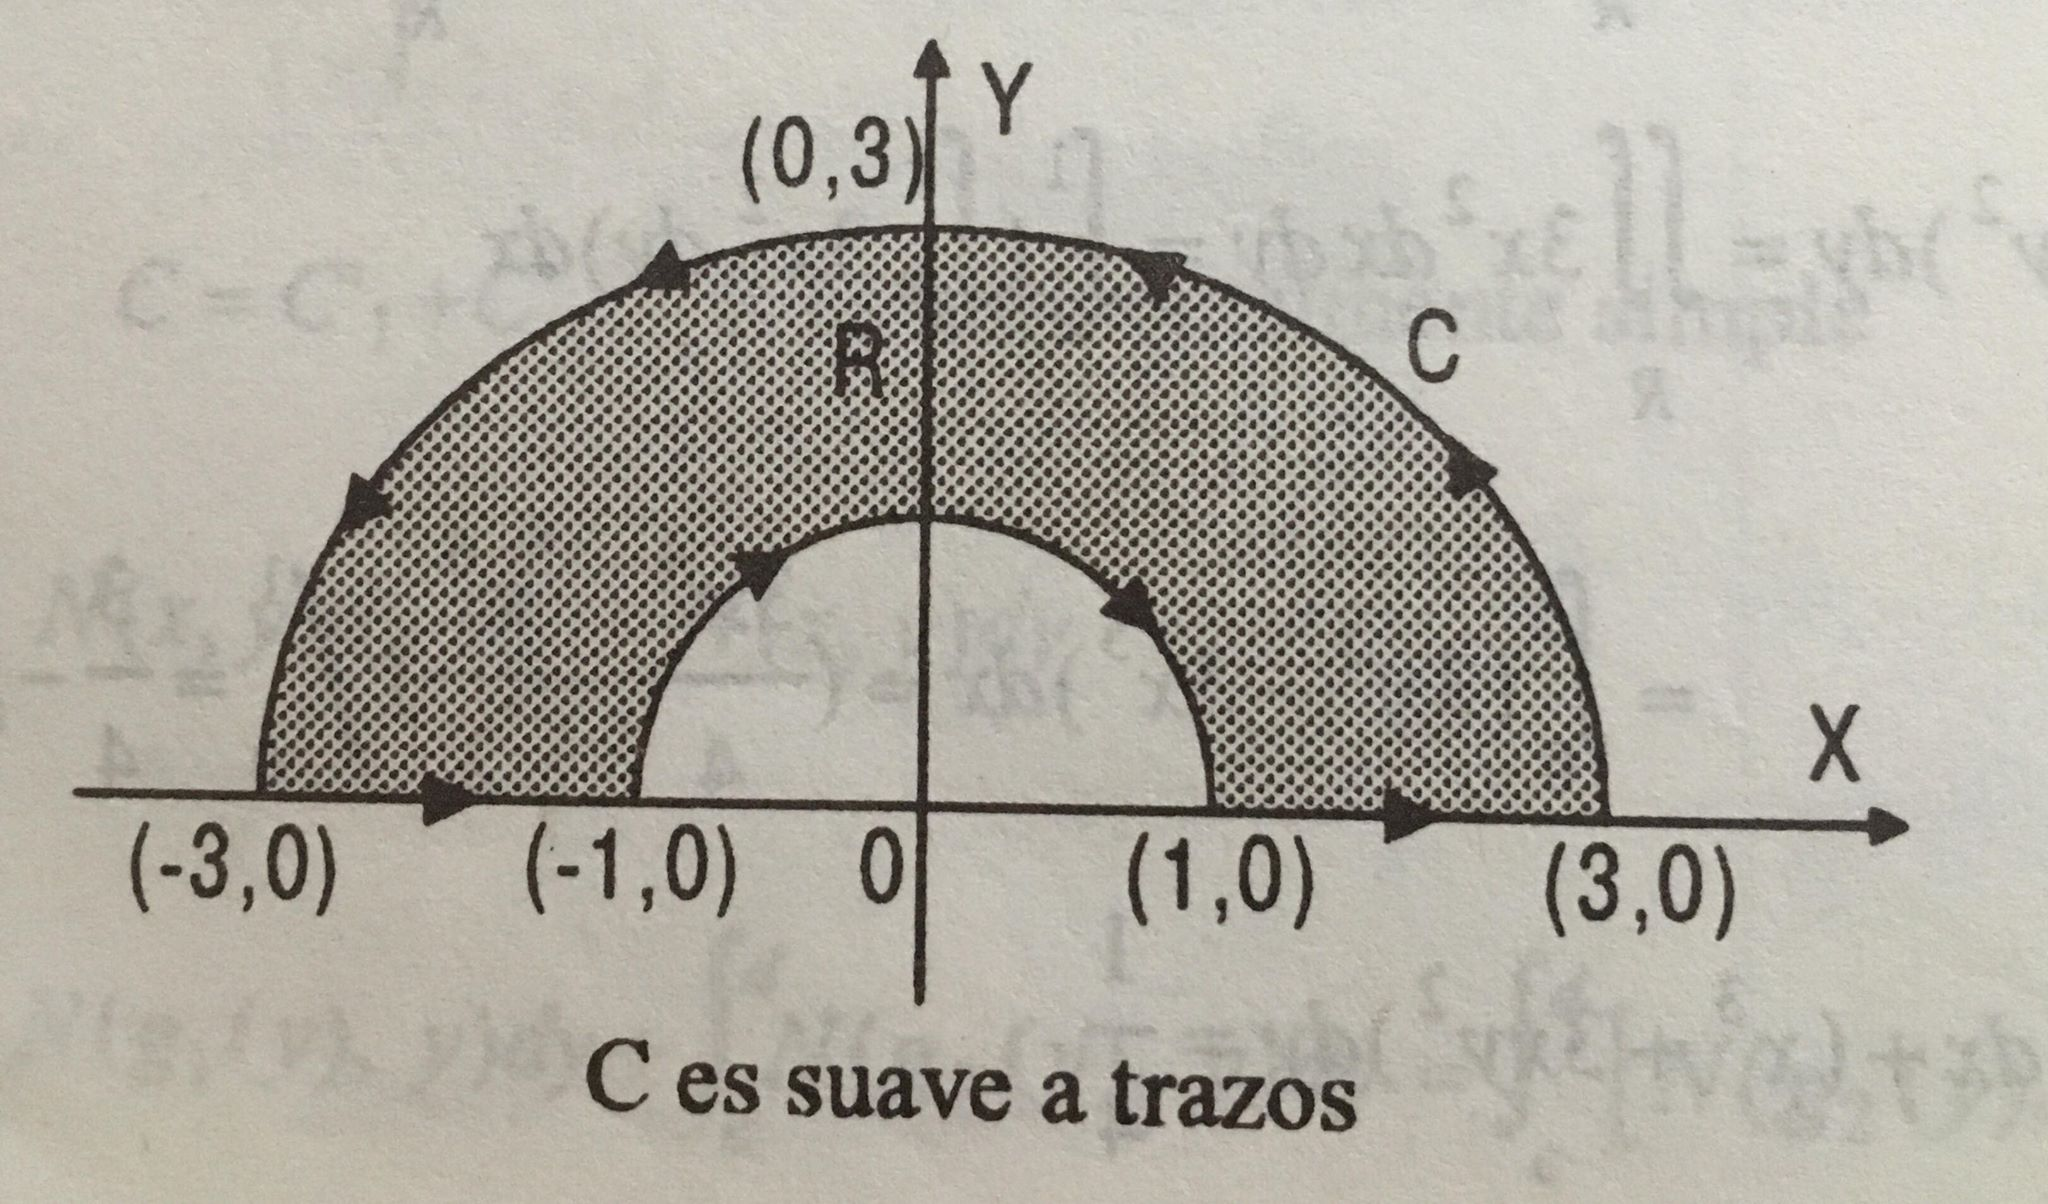
\includegraphics[width=0.6\linewidth,angle=0]{Figura1.jpg}
		\end{center}
	\end{figure}\\
    problema xx, pag. 828, Calculo 3 Eduardo Espinoza
\end{itemize}
\begin{itemize}
	\item [15.] Ache a área da superfície $S$ que é a parte da esfera $x^{2}+y^{2}+z^{2}=1$ dentro do cone $x^{2}+y^{2}=z^{2}$, para $z>0$.\\
	problema 3.14, pag. 413, Venero
\end{itemize}
\begin{itemize}
	\item [16.] Calcule a integral do campo vetorial $F(x,y,z)= 2(x,y,z)$ sobre o hemisfério $S$: $x^{2}+y^{2}+z^{2}=a^{2}$, $a>0$, $z\geqslant 0$.\\
	problema 6.2, pag. 436, Venero 
\end{itemize}
\begin{itemize}
	\item [17.] Calcule a massa da chapa fina $\sigma$ dada por $x=u$, $y=v$ e $z=u+2v$, $0\leqslant u\leqslant 1$ e $0\leqslant v\leqslant1$, sendo $f(x,y,z)=x+y+z$ a densidade superficial.\\
	problema 2, pag. 217, Guidozzi, vol 3
\end{itemize}

\begin{itemize}
	\item [18.]  Verifique o Teorema de Stokes 
	\begin{itemize}
	\item[a.] Para o campo vetorial $F(x,y,z)=(2xy,2-x-3y,x^{2}+z)$, sobre o lado exterior da superfície $S$ da interseção de dois cilindros $x^{2}+y^{2}=a^{2}$, $x^{2}+z^{2}=a^{2}$ ($a>0$) situado no primeiro quadrante.\\
	problema 10.3 pag. 498 Venero.
	\item[b.] Para o campo vetorial $F(x,y,z)=(y,-x,0)$ sobre o paraboloide $S: z=x^{2}+y^{2}$ com a circunferência $x^{2}+y^{2}=1$, $z=1$, como seu borda $\partial S$.\\
	problema 10.2 pag. 497 Venero.
   \end{itemize}
\end{itemize}
\begin{itemize}
	\item [19.] Calcule p fluxo do rotacional de $F(x,y,z)=(x,y,xyz)$ através da superficie $z=1+x+y, x\geqslant 0, y\geqslant 0$ e $x+y\leqslant 1$, como normal $n$ apontando para baixo.\\
	problema 4, pag. 257, Guidorizzi Vol 3  
\end{itemize}
\begin{itemize}
	\item [20.] Seja $F(x,y,z)=(x^{2}y,xy^{2},(5-4xyz))$ e seja $\sigma$ a superfície $x^{2}+y^{2}+z^{2}=4$, $z\geqslant 0$, sendo $n$ normal a $\sigma$ com componente $z>0$. Calcule o fluxo de $F$ através de $\sigma$, na direção $n$.\\
	problema 2, pag. 235, Guidorizzi Vol 3  
\end{itemize}
\begin{itemize}
\item [21.] Seja $E(x,y,z)=\frac{q}{(x^{2}+y^{2}+z^{2})\sqrt{x^{2}+y^{2}+z^{2} }} (x,y,z)$; 
\begin{itemize}
	\item[a.] Calcule $\div (F)$.
	\item[b.] Calcule o fluxo de $E$ através da superfície esférica $ x^{2}+y^{2}+z^{2}=1$, com normal $n$ apontando para fora da esfera $x^{2}+y^{2}+z^{2} \leqslant 1$.
	\item[c.] Calcule o fluxo de $E$ através da superfície $x^{2}+y^{2}+(z-2)^{2}=1$,  com normal $n$ apontando para fora da esfera $x^{2}+y^{2}+(z-2)^{2} \leqslant 1$ .
	\item[d.] Calcule o fluxo de $E$ através da fronteira do cubo $-2 \leqslant x\leqslant2$,$-2 \leqslant y\leqslant2$, $-2 \leqslant z\leqslant2$ com normal $n$ apontando para fora do cubo.
\end{itemize}
problema 3, pag. 237, Guidorizzi Vol 3.
\end{itemize}
\end{document}
